\subsubsection{Admission control for Multiple LQs}
\label{sec:admission_sim}

\begin{figure}[!h]
    \centering
    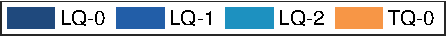
\includegraphics[width=0.8\linewidth]{fig/res_usage_b1i3_legend} 
    \vspace{-0.2cm}
    \subfloat[DRF: \burstq-0, \burstq-1, \burstq-2 are unhappy with high latency.]{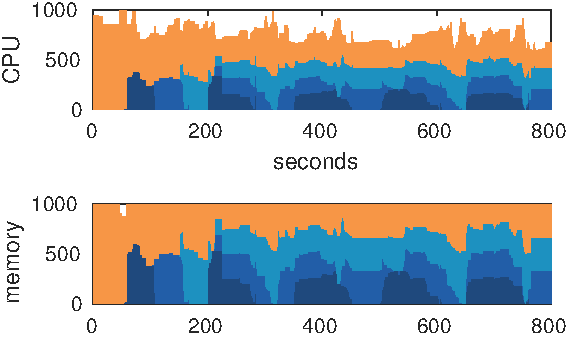
\includegraphics[width=0.8\linewidth]{fig/b1i3_res_usage_drf} \label{fig:admission_drf}} 
    \vspace{-0.1cm}
    \subfloat[SP: \batchq-0 is starving of resources.]{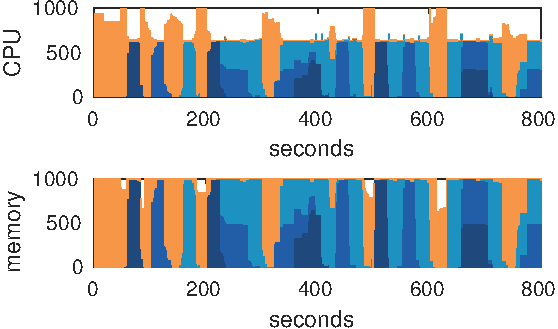
\includegraphics[width=0.8\linewidth]{fig/b1i3_res_usage_strict} \label{fig:admission_strict}}
    \vspace{-0.1cm}            
    \subfloat[N-\name: Only {\burstq}-0 and {\batchq}-0 are happy.]{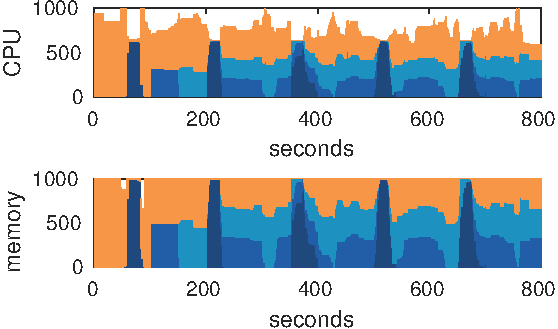
\includegraphics[width=0.8\linewidth]{fig/b1i3_res_usage_Hard} \label{fig:admission_hard}}
    \vspace{-0.1cm}    
    \subfloat[\name: {\burstq}-0, {\burstq}-1 and {\batchq}-1 are happy.]{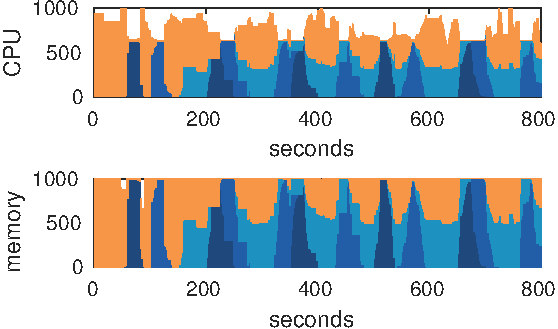
\includegraphics[width=0.8\linewidth]{fig/b1i3_res_usage_speedfair} \label{fig:admission_speedfair}}
    \vspace{-0.1cm}    
    \caption{[Simulation] DRF and SP fail to guarantee both performance and fairness simultaneously. \name gives the best performance to \burstq-0, near optimal performance for \burstq-1, and maintains fairness among 4 queues. \burstq-2 requires too much resource, so its performance cannot be guaranteed.}
    \vspace{-0.5cm}    
    \label{fig:admission_control}
\end{figure}


To demonstrate how \name works with multiple {\burstq}s, we set up 3 {\burstq}s (\burstq-0, \burstq-1, and \burstq-2) and a single \batchq (TQ-0).
The jobs \batchq-0 are queued up at the beginning while \burstq-0, \burstq-1, and \burstq-2 arrive at 50, 100, and 150 seconds, respectively.
The periods of {\burstq}-0, {\burstq}-1, and {\burstq}-2 are 150, \diff{110}, and 60 secs. All the {\burstq}s jobs have the identical demand and task durations.
The TQ jobs are chosen from the BB benchmark.
\name admits {\burstq}-0 to the Hard Guarantee class, {\burstq}-1 to the Soft Guarantee class, and {\burstq}-2 to the Elastic class.

Figure \ref{fig:admission_control} shows the resource usage (CPU and memory) for each queue across four schedulers, i.e., DRF, SP, N-\name and \name.
The capacity of CPU or memory is 1000 nodes.
As an instantaneously fair scheduler, DRF continuously maintains the fair share for all queues as in Figure \ref{fig:admission_drf}.
Since \burstq-2 requires a lot of resources, SP makes \batchq-0 starving for resources (Figure \ref{fig:admission_strict}). N-\name provides \burstq-0 with resource guarantee and it fairly share the resources to \burstq-1, \burstq-2, and \batchq-0 (Figure \ref{fig:admission_hard}).
\name provides hard guarantee to \burstq-0 and soft guarantee to \burstq-1 as in Figure \ref{fig:admission_speedfair}.
The soft guarantee allows \burstq-1 performs better than using N-\name.
Since \burstq-2 demands too much resources, \name treats it like \batchq-0.

Figure \ref{fig:avg_multi_queue} shows the average completion time of jobs on each queue across the four schedulers.
The performance of DRF for \burstq jobs is the worst among the four schedulers but it is the best for only \batchq-0.
The performance of SP is good for \burstq jobs but it is the worst for \batchq jobs.
N-\name provides the best performance for \burstq-0 but not \burstq-1 and \burstq-2.
\name is the best among the four schedulers.
The three of four queues, i.e., \burstq-0, \burstq-1, and \batchq-0, significantly benefit from \name.
\name even outperforms SP for \burstq-0 and \burstq-1 jobs and does not hurt any {\batchq}.

\begin{figure}[!h]
    \centering
    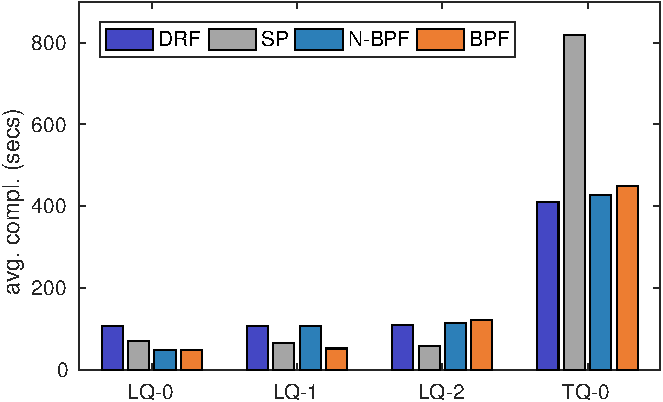
\includegraphics[width=0.8\linewidth]{fig/avg_multi_queuesadmit}
    \caption{[Simulation] \name provides with better performance for {\burstq}s than DRF and N-\name. Unlike SP, \name protects the performance of \batchq jobs.}
    \label{fig:avg_multi_queue}
\end{figure}
